\documentclass[10pt,journal]{article}

% Portable drafting template. Convert to the target venue template before submission.
\usepackage[utf8]{inputenc}
\usepackage{graphicx}
\usepackage{booktabs}
\usepackage{amsmath}
\usepackage{url}
\usepackage[hidelinks]{hyperref}
\usepackage{geometry}
\geometry{margin=1in}

\title{An Empirical Study of Bug Types in LLM-Generated Code:\\
A Taxonomy and Cross-Model Analysis}
\author{Zixiao Xie\\
School of Information Sciences, University of Illinois Urbana-Champaign\\
\texttt{zixiaox2@illinois.edu}}
\date{\today}

\begin{document}
\maketitle

\begin{abstract}
Large language models (LLMs) are used to generate source code, yet
evaluation has largely focused on aggregate functional correctness, such as pass@k.
Comparatively little is known, systematically, about the kinds of bugs that arise
when generated code fails. This paper presents a reproducible empirical pilot study
that derives a bug taxonomy, quantifies bug-type frequencies, and compares
distributions across four hosted models. We evaluate GPT-4o-mini, DeepSeek-Chat,
Qwen2.5-72B-Instruct, and Llama-3.1-8B-Instruct on the 164-problem HumanEval
benchmark. Across 656 generations, 110 fail the unit tests. In this sample,
LOGIC failures account for 87.3\% of failures: the generated code executes but
returns a wrong result (95\% Wilson CI: 79.8--92.3\%). Refining the logic-error
category into seven subtypes finds that mathematical-reasoning errors (44.8\%,
43/96; 95\% CI: 35.2--54.7\%) and wrong-algorithm choices (21.9\%, 21/96;
95\% CI: 14.8--31.1\%) together account for 64/96 (66.7\%) of LOGIC failures.
A chi-square test finds no
statistically significant association between model and bug-type composition
($\chi^2=21.29$, $p=0.27$). We release the pipeline, prompts, labels, and analysis scripts as
supplementary material. Because labels are currently machine-assigned, we frame the
study as a reproducible pilot. An independent blind LLM annotator yields fair
agreement with the primary subtype labels (Cohen's $\kappa=0.305$), indicating that
fine-grained subtype labels should be interpreted cautiously; human
validation and multi-benchmark replication remain future work.
\end{abstract}

\textbf{Keywords:} large language models, code generation, software bugs,
empirical software engineering, taxonomy, research software.

\section{Introduction}
LLM-based code assistants are now used in software development. A common way to
measure their coding ability is functional correctness on
benchmarks such as HumanEval~\cite{chen2021codex} and MBPP~\cite{austin2021mbpp}.
Such metrics quantify how often models succeed, but they say little about how
models fail. For practitioners who must review and repair AI-generated code, the
type of mistake matters: a wrong output format is cheap to fix, while a subtle
logic error may pass superficial review.

This paper asks:
\begin{itemize}
  \item \textbf{RQ1.} What categories of bugs occur in LLM-generated code, and what
  is the frequency distribution of each category?
  \item \textbf{RQ1b.} Within the observed LOGIC class, what subtype of reasoning
  error is responsible?
  \item \textbf{RQ2.} Do bug-type distributions differ significantly across models?
\end{itemize}

\noindent\textbf{Contributions.}
(1) A reproducible pipeline that turns benchmark generations into a labeled bug
dataset; (2) an execution-grounded failure dataset for four hosted models on
HumanEval; (3) a two-level analysis that separates coarse bug categories from
finer LOGIC subtypes; (4) an independent blind automatic agreement check for the
subtype labels; and (5) a software artifact intended for reuse and extension.

\section{Related Work}
\textbf{Functional evaluation of code LLMs.}
HumanEval~\cite{chen2021codex} and MBPP~\cite{austin2021mbpp} established
execution-based benchmarks. EvalPlus~\cite{liu2023evalplus} showed that augmented
tests expose additional failures, and SWE-bench~\cite{jimenez2024swebench} extends
evaluation to repository-level issues. Later benchmarks broaden the evaluation
setting across languages and more realistic tasks, including MultiPL-E's polyglot
extension~\cite{cassano2023multipl}, LiveCodeBench's contamination-aware
time-sliced evaluation~\cite{jain2024livecodebench}, and DevEval's repository-style
tasks~\cite{li2024deveval}. These efforts measure whether code is correct, or
whether models solve increasingly realistic programming tasks, but they do not
primarily explain the nature of the errors once code fails.

\textbf{Characterizing LLM code errors.}
Closest to this work, Tambon et al.~\cite{tambon2024bugs} conduct a large empirical
study of bugs in LLM-generated code and provide a published baseline for bug
taxonomy work. We therefore do not claim that taxonomy-based analysis of
LLM-generated code is new. Instead, our contribution is narrower and artifact
oriented. We focus on a compact, reproducible HumanEval pipeline whose intermediate
artifacts are released with the analysis: raw generations, executable failure signals,
primary labels, LOGIC subtype labels, agreement outputs, tables, figures, and an
arXiv-ready manuscript package. Methodologically, we separate coarse failure
categories from a second-stage analysis of the observed LOGIC class and report an
independent blind LLM-vs-LLM agreement check for those fine-grained subtype labels.
This frames the present work as a reproducible pilot and research-software
artifact that complements broader empirical studies rather than replacing them.

\section{Methodology}
\subsection{Benchmark and Generations}
We use HumanEval~\cite{chen2021codex}, which contains 164 Python problems with
unit tests. We query four instruction-tuned models through a uniform prompt:
\texttt{openai/gpt-4o-mini}, \texttt{deepseek/deepseek-chat},
\texttt{qwen/qwen-2.5-72b-instruct}, and
\texttt{meta-llama/llama-3.1-8b-instruct}. Generation uses temperature $0.2$, one
sample per problem, and a $1024$-token limit. The recorded access date for the
current artifact is 2026-06-23. Machine-readable model, provider, generation, and
labeler metadata are included in the released artifact as
\texttt{results/tables/model\_metadata.csv}.

\subsection{Failure Identification}
Each generation is sanitized and executed against the problem's test suite in an
isolated subprocess with a timeout. A generation is a failure if it does not pass.
The harness is validated by confirming that all 164 canonical solutions pass.

\subsection{Bug Taxonomy and Labeling}
We label each failure with exactly one primary category (Table~\ref{tab:taxonomy}).
Deterministic failure signals such as syntax errors, timeouts, and exception types
are mapped by rule. Assertion failures are assigned by an LLM classifier because
the code runs but returns a wrong result.

Because LOGIC is the largest failure category in this sample, we further label
LOGIC failures into seven subtypes (Table~\ref{tab:subtaxonomy}). The primary subtype classifier sees the
problem specification, the buggy code, and the reference solution to aid root-cause
attribution. To reduce over-reliance on a single classifier, the repository also
includes an independent blind second annotator that uses a different model and does
not see the reference solution, primary label, or primary explanation. Agreement is
reported as LLM-vs-LLM Cohen's $\kappa$~\cite{cohen1960kappa}. This automatic
agreement analysis is a robustness check, not a replacement for human validation.
For later manual validation, the artifact also includes a deterministic 40-item
blind review sheet and coding guide; its human-label fields are blank in the
current release.

\begin{table}[t]
\centering
\caption{Bug-type taxonomy.}
\label{tab:taxonomy}
\small
\begin{tabular}{ll}
\toprule
Code & Definition \\
\midrule
LOGIC & Algorithmic/logic error; runs but wrong result \\
BOUNDARY & Fails on edge/special inputs \\
SPEC & Misunderstood the specification \\
FORMAT & Right idea, wrong return shape/format \\
API\_MISUSE & Nonexistent or misused API \\
TYPE & Type mismatch or wrong argument arity/order \\
INCOMPLETE & Stub or missing branch \\
TIMEOUT & Infinite loop or excessive runtime \\
SYNTAX & Does not parse \\
OTHER & None of the above \\
\bottomrule
\end{tabular}
\end{table}

\begin{table}[t]
\centering
\caption{Refined subtaxonomy of LOGIC errors.}
\label{tab:subtaxonomy}
\small
\begin{tabular}{ll}
\toprule
Subtype & Definition \\
\midrule
Wrong algorithm & Wrong overall approach; a different method is needed \\
Missing edge case & Unhandled special input \\
Boundary condition & Off-by-one, first/last, inclusive vs. exclusive \\
State/update error & Wrong accumulator, counter, or in-place update \\
Math reasoning & Wrong formula, operation, rounding, sign, or carry \\
Premature simplification & Ignored a stated requirement; over-simplified \\
Spec partial impl. & Only some required cases/branches implemented \\
\bottomrule
\end{tabular}
\end{table}

\subsection{Analysis}
We report per-model pass rates, overall category frequency, refined LOGIC subtype
frequency, and 95\% Wilson confidence intervals for binomial proportions. We also
report a category-by-model contingency table tested with a chi-square test of
independence, plus a lower-dimensional LOGIC/non-LOGIC companion test.

\section{Results}
Across $4 \times 164 = 656$ generations, 546 (83.2\%) pass and 110 fail. Per-model
pass rates are: DeepSeek-Chat 93.3\%, GPT-4o-mini 87.8\%, Qwen2.5-72B 86.6\%, and
Llama-3.1-8B 65.2\%.

\begin{table}[t]
\centering
\caption{Per-model pass rate on HumanEval ($n=164$ each).}
\label{tab:pass}
\small
\begin{tabular}{lrr}
\toprule
Model & Pass rate (\%) & 95\% CI \\
\midrule
DeepSeek-Chat & 93.3 & 88.4--96.2 \\
GPT-4o-mini & 87.8 & 81.9--92.0 \\
Qwen2.5-72B-Instruct & 86.6 & 80.5--91.0 \\
Llama-3.1-8B-Instruct & 65.2 & 57.7--72.1 \\
\bottomrule
\end{tabular}
\end{table}

\subsection{RQ1: Bug-Type Distribution}
\label{sec:rq1}
Figure~\ref{fig:freq} shows the distribution of bug types over the 110 failures.
LOGIC errors account for 87.3\% (96/110; 95\% CI: 79.8--92.3\%) of all failures.
The remaining failures are spread thinly across API\_MISUSE (4.5\%), TYPE (3.6\%),
BOUNDARY (1.8\%), and a long tail of SPEC, SYNTAX, and OTHER.

\begin{figure}[t]
\centering
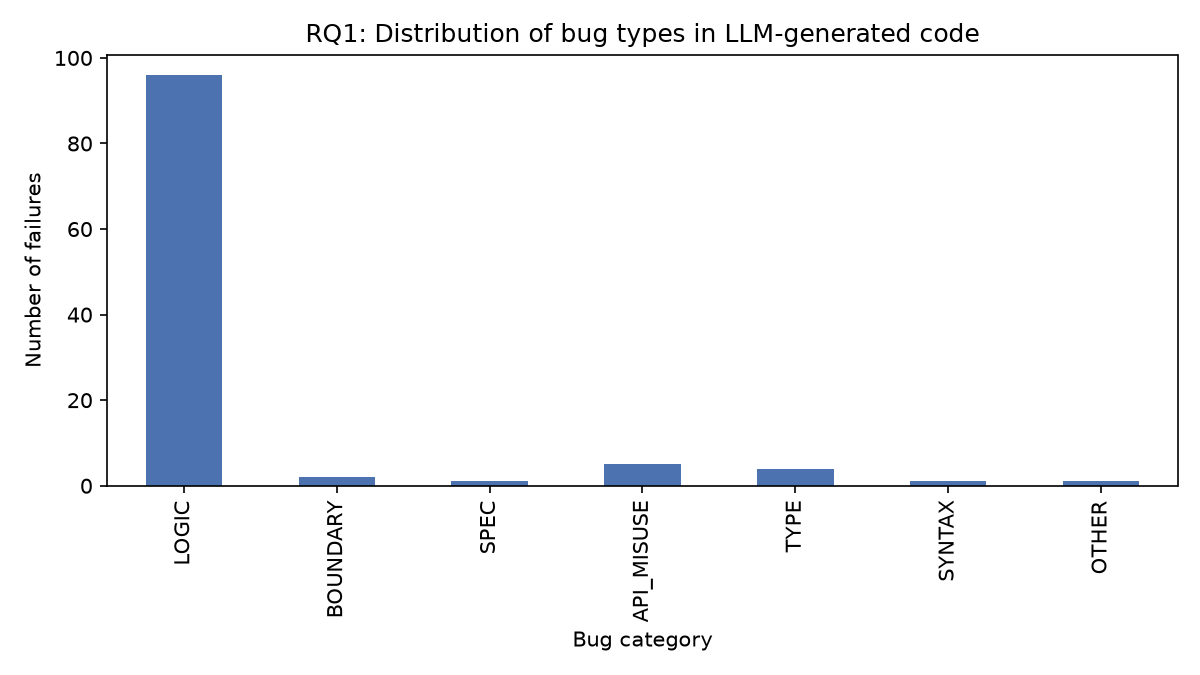
\includegraphics[width=0.95\linewidth]{../results/figures/fig1_category_freq.png}
\caption{Distribution of bug types across all 110 failing generations.}
\label{fig:freq}
\end{figure}

\subsection{RQ1b: Logic Subtypes}
\label{sec:rq1b}
Figure~\ref{fig:logicsub} breaks the 96 LOGIC failures into seven subtypes. The
largest subtype is mathematical-reasoning errors (44.8\%, 43/96; 95\% CI:
35.2--54.7\%), followed by wrong-algorithm choices (21.9\%, 21/96; 95\% CI:
14.8--31.1\%) and missing edge cases (16.7\%, 16/96). Together, these results
indicate that most observed LOGIC failures involve problem reasoning rather than
parse errors, crashes, or simple API misuse.

\begin{figure}[t]
\centering
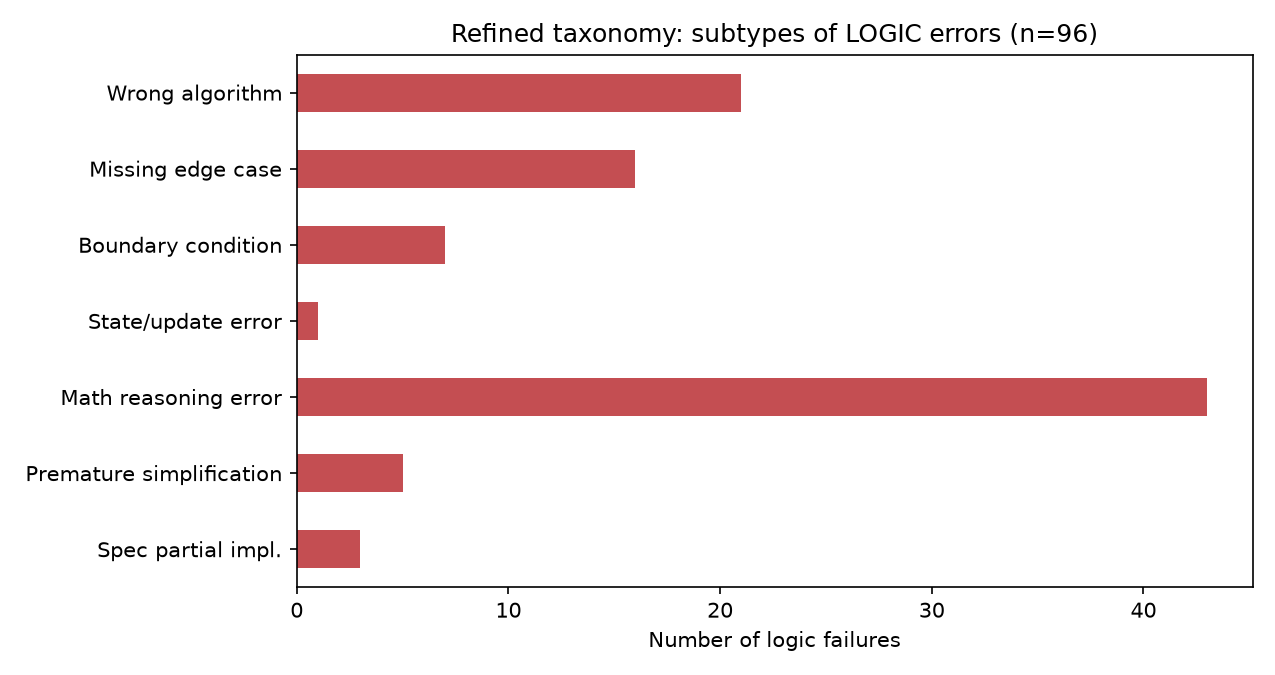
\includegraphics[width=0.95\linewidth]{../results/figures/fig3_logic_subcat.png}
\caption{Refined breakdown of the 96 LOGIC failures into seven subtypes.}
\label{fig:logicsub}
\end{figure}

\subsection{RQ2: Variation Across Models}
A chi-square test of independence on the category-by-model contingency table does
not detect an association ($\chi^2=21.29$, $\mathrm{dof}=18$, $p=0.27$), with Cramer's
$V=0.254$. Because the contingency table is sparse (24/28 expected cells are below
5), we treat this test as exploratory rather than definitive. A deterministic
10{,}000-iteration permutation check gives a similar result ($p=0.2691$). A companion
LOGIC/non-LOGIC test also does not detect an association ($\chi^2=3.394$, $\mathrm{dof}=3$,
$p=0.335$, Cramer's $V=0.176$), although 3/8 expected cells remain below 5; its
permutation p-value is 0.3445. In this sample, models differ in how often they
fail, but we do not detect a reliable difference in how they fail.

\begin{figure}[t]
\centering
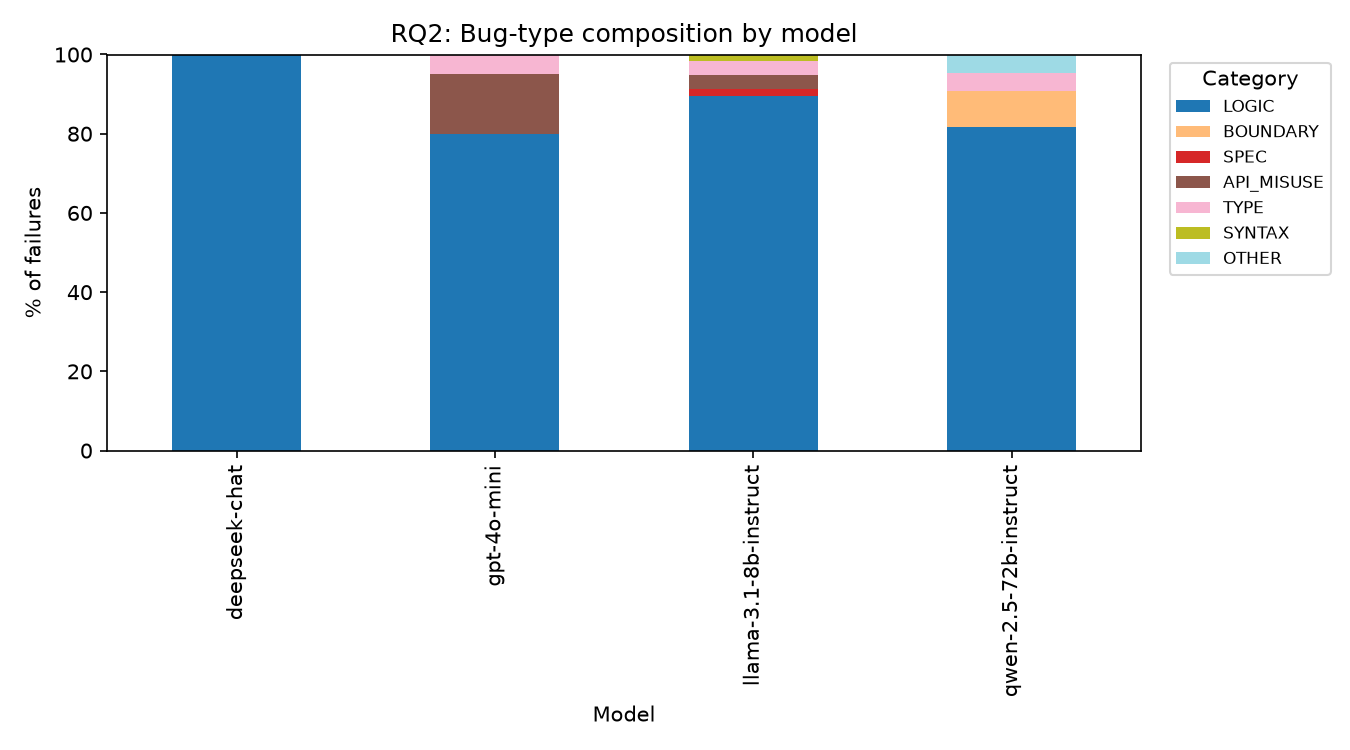
\includegraphics[width=0.95\linewidth]{../results/figures/fig2_category_by_model.png}
\caption{Bug-type composition by model.}
\label{fig:bymodel}
\end{figure}

\subsection{Automatic Label-Agreement Check}
To assess the stability of the LOGIC subtype labels, we run an independent blind
second LLM annotator on all 96 LOGIC failures. The blind annotator does not see the
reference solution, the primary subtype label, or the primary explanation. Exact
agreement is 42/96 (43.8\%), and Cohen's $\kappa$ is 0.305, conventionally
interpreted as fair agreement. This result is not strong enough to treat the
subtype labels as fully validated. Instead, the coarse LOGIC/non-LOGIC distinction
is better supported by the current evidence than the finer distinction between,
for example, mathematical reasoning, wrong algorithm, and partial specification
implementation.

\section{Discussion}
\textbf{Most failures in this sample are executable wrong-output failures.}
Syntax and crash errors are infrequent in the observed failure set. More often,
generated code runs but implements the wrong computation.

\textbf{The refined categories point to reasoning-related review work.}
Mathematical-reasoning and wrong-algorithm errors are the largest LOGIC subtypes.
For this dataset, semantic checks, edge-case tests, and differential tests are
more directly aligned with the observed failures than checks limited to syntax or
runtime exceptions.

\textbf{Failure rates differ more clearly than failure profiles.}
The exploratory RQ2 results show clearer variation in pass rate than in category
composition across the four models. Because both the full-category and
LOGIC/non-LOGIC tests have sparse expected cells, this should be read as a
hypothesis for replication rather than a settled claim.

\section{Threats to Validity}
\label{sec:threats}
\textbf{Construct validity.} Bug type is partly subjective. Current labels are
machine-assigned, and the primary subtype classifier sees the reference solution.
The independent blind second annotator provides an automatic robustness check, but
the resulting fair agreement ($\kappa=0.305$) shows that fine-grained subtype
boundaries remain uncertain. LLM-vs-LLM agreement does not replace human
validation. The release includes a 40-item blind human-review instrument, but no
human-validation result is reported because the human label fields are not filled.

\textbf{External and statistical validity.} Results are limited to Python,
HumanEval, low temperature, and one sample per problem. The full category-by-model
test is sparse, and the LOGIC/non-LOGIC companion test still has some expected
cell counts below 5, so the RQ2 comparison is best interpreted as exploratory.
Replication on MBPP, additional languages, and multiple samples is needed.

\textbf{Reproducibility.} Code, prompts, generated outputs, labels, and analysis
scripts are provided. Hosted model identifiers may route to provider-current
weights, so exact regeneration can depend on provider stability.

\section{Conclusion}
This paper presents a reproducible empirical pilot study of bug types in
LLM-generated code. In the studied HumanEval sample, most failures are
wrong-output LOGIC errors rather than crashes or syntax errors. Within those LOGIC errors,
mathematical-reasoning and wrong-algorithm failures are the two largest subtypes,
though independent automatic agreement indicates that fine-grained subtype
boundaries should be treated as exploratory. The next steps are to add human
validation where possible, scale to more samples and benchmarks, and package the
software artifact for reuse.

\bibliographystyle{plain}
\bibliography{references}
\end{document}
